\documentclass[compsoc]{IEEEtran}
\usepackage{graphicx}
\usepackage{amsmath}
\usepackage{authblk}
\usepackage[english]{babel}
\usepackage{blindtext}
%\usepackage[ruled,vlined,linesnumbered]{algorithm2e}
%\usepackage{algorithmic,float}
\usepackage{setspace}
\usepackage{amsfonts}
\usepackage{hyperref}
\graphicspath{ {./images/} }
\usepackage{subfig}
\usepackage{fontspec}
\usepackage{listings}
\usepackage{amsmath}
\usepackage{mathabx}
\usepackage[bottom]{footmisc}
\newfontfamily\listingsfont[Scale=.7]{inconsolata}\usepackage[font=footnotesize,labelfont=bf]{caption}
%\captionsetup[algorithm2e]{font=footnotesize}
\usepackage[table,xcdraw]{xcolor}
\usepackage[utf8]{inputenc}
\title{Assignment: CNN and MNIST}
\author{David Bertoldi -- 735213 \\ email: d.bertoldi@campus.unimib.it}
\affil{Department of Informatics, Systems and Communication}
\affil{University of Milano-Bicocca}
\date{October 2022}


\begin{document}

\maketitle 



\section{Inspecting the data}
The MNIST dataset contains 70,000 images of handwritten digits (zero to nine) that have been size-normalized and centered in a square grid of pixels. Each image is a 28 × 28 × 1 array of floating-point numbers representing grayscale intensities ranging from 0 (black) to 1 (white). The target data consists of one-hot binary vectors of size 10, corresponding to the digit classification categories zero through nine. Figure \ref{fig:hist} shows the data distribution for both training and test datasets.

\begin{figure}[ht!]
\centering                                                                        
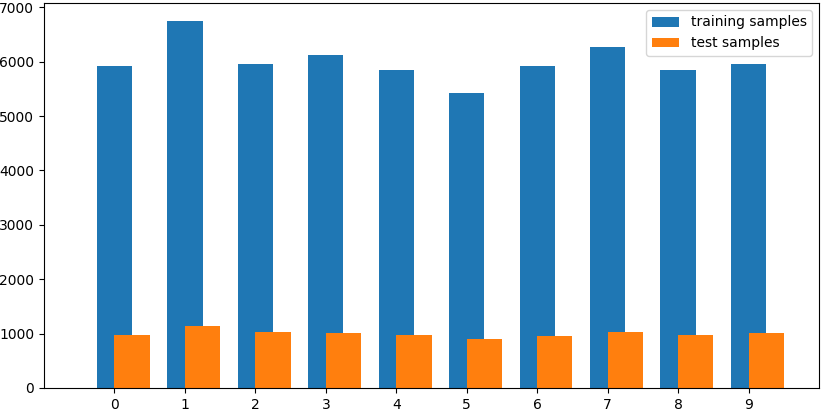
\includegraphics[width=3.5in]{hist.png}
\captionsetup{justification=centering}                                                                                                                                   
\caption{Histogram of the dataset}
\label{fig:hist}                                                                                                                                                           
\end{figure}


The training population presents a distribution with mean $\mu = 6\,000$ and standard deviation $\sigma \simeq 340$ and thus we didn't notice any important unbalance in the data.

\section{Preparing the data}

\section{Building the network and training}
\subsection{Data split}


\subsection{Network}



\end{document}









